\documentclass[12pt]{paper}

\usepackage[utf8]{inputenc}
\usepackage[T1]{fontenc}

\usepackage[margin=1in]{geometry}
\usepackage{amsmath}
\usepackage{bm}
\usepackage{amsthm}
\usepackage{mathtools}
\usepackage{amsfonts}
\usepackage{bbm}
\usepackage{graphicx}
\usepackage{minted}

\usepackage{longtable}
\usepackage{wrapfig}
\usepackage{rotating}
\usepackage[normalem]{ulem}
\usepackage{amsmath}
\usepackage{textcomp}
\usepackage{amssymb}
\usepackage{capt-of}
%\usepackage{hyperref}
\usepackage{tikz}
\usepackage{bm}
\usepackage{minted}

\usepackage{amsmath}
\usepackage{bm}
\usepackage{amsthm}
\usepackage{mathtools}
\usepackage{amsfonts}
\usepackage{bbm}
\usepackage{graphicx}

\usepackage{fontspec}
\setmonofont{Ubuntu Mono}


\DeclareMathOperator{\diam}{diam}
\DeclareMathOperator{\interior}{int}
\DeclareMathOperator{\close}{cl}

\newcommand{\met}[1]{d \left ( #1 \right )}
\newcommand{\brak}[1]{ \left [ #1 \right ] }
\newcommand{\cbrak}[1]{ \left \{ #1 \right \}}
\renewcommand{\vec}[1]{ \bm{ #1 }}
\newcommand{\abs}[1]{\left \lvert #1 \right \rvert}
\newcommand{\seq}[1]{{\left \{ #1 \right \}}}
\newcommand{\conj}[1]{ \overline{ #1 } }
%\newcommand{\close}[1]{ \bar{ #1 } }
\newcommand{\set}[1]{\left \{ #1 \right \}}
\newcommand{\Lim}{\lim\limits}
\newcommand{\compose}{\circ}
\newcommand{\inv}[1]{{#1}^{-1}}
\newcommand{\compl}[1]{{#1}^{c}}



\newcommand{\setR}{ \mathbb{R} }
\newcommand{\setQ}{ \mathbb{Q} }
\newcommand{\setZ}{ \mathbb{Z} }
\newcommand{\setN}{ \mathbb{N} }

\newcommand{\plim}{ \overset{p}{\to} }
\newcommand{\mean}[2][N]{ \overline{ #2 }_{#1}}
\newcommand{\exV}[1]{\mathbb{E} \left [ #1 \right ]}
\newcommand{\Vari}[1]{\mathbb{V} \left ( #1 \right )}

\newcommand{\est}[2][n]{ \widehat{ #2 }_{#1}}
\newcommand{\altest}[2][n]{ \tilde{ #2 }_{#1}}

\newcommand{\indicate}[1]{ \mathbbm{1}_{\{#1\}}}
\newcommand{\convDist}{ \overset{d}{\to}}
\newcommand{\unif}{\emph{U}}
\newcommand{\normal}{\mathcal{N}}
\newcommand{\eye}{\mathbbm{I}}

\newcommand{\bigO}{\mathcal{O}}
\newcommand{\Lagrange}{\mathcal{L}}

\newcommand{\deriv}[2]{\frac{ \partial #1}{ \partial #2}}

\DeclarePairedDelimiter{\ceil}{\lceil}{\rceil}
\DeclarePairedDelimiter{\floor}{\lfloor}{\rfloor}
\DeclarePairedDelimiter{\norm}{\lVert}{\rVert}

\author{Timothy Schwieg}
\date{\today}
\title{Optimization Conscious Econometrics Pset 2 Part 2}

\begin{document}

\maketitle

\section{Write the likelihood for model (1) with both logit and linear
  links}

\subsection{Linear Link}

For the linear link, we note that $x_{i,t}\beta$ is a constant, and that
$\alpha_i \sim \normal(0,\tau^2)$ so $x_{i,t}\beta + \alpha_i \sim \normal( x_{i,t}\beta, \tau^2)$.

However, for each observation for person $i$, there is the same draw
of $\alpha_i$. The object in question is $x_i \beta + 1 \alpha_i$ where
$1_T$ is a $T$-dimensional vector containing all ones, and $x_i$ is
the vector containing all $T$ measurements from consumer $i$.

The joint distribution of this object is given by:
\begin{equation*}
 x_i \beta + 1_T \alpha_i \sim \normal(x_i \beta, \tau^2 1_T 1_T' ) 
\end{equation*}

Letting $\Sigma = \tau^2 1_T 1_T'$


The Likelihood function is simply the product of the densities
evaluated at their outcomes.

\begin{equation*}
  L = \prod_{i=1}^n \frac{1}{\sqrt{2 \pi \abs{\Sigma}}} \exp (
  -\frac{1}{2} (y_i - x_i)' \inv{\Sigma} (y_i - x_i) )
\end{equation*}


\subsection{Logit Link Function}

I invert the logit link function so that we reach the model where
$y_{i,t} = g( x_{i,t}\beta + \alpha_i)$ where

\begin{equation*}
  g(y) =
  \begin{pmatrix}
    \frac{\exp(y_1)}{1+\exp(y_1)}\\
    ...\\
    \frac{\exp(y_t)}{1+\exp(y_t)}\\
    ...\\
    \frac{\exp(y_T)}{1+\exp(y_T)}
  \end{pmatrix}
\end{equation*}

This is a bijection from $\setR^T \rightarrow (0,1)^T$. As such we can define
the inverse mapping $\inv{g}$.

\begin{equation*}
  \inv{g}(y) =
  \begin{pmatrix}
    \log \left( \frac{y_1}{1-y_1} \right)\\
    ...\\
    \log \left( \frac{y_t}{1-y_t} \right)\\
    ...\\
    \log \left( \frac{y_T}{1-y_T} \right)
  \end{pmatrix}
\end{equation*}


Note that $\frac{\exp(y_i)}{1 + \exp(y_i)} = 1 -
\frac{1}{1+\exp(y_i)}$. Its derivative is $g(x)(1-g(x))$
The Jacobian of the transformation $g(x)$ is given by:

\begin{equation*}
  J =
  \begin{pmatrix}
    g(y_1)(1-g(y_1)) & 0 & ... & 0\\
    0 & g(y_2)(1-g(y_2)) & ... & 0 \\
    ... & & &\\
    0 & 0 & ... & g(y_T)(1-g(y_T))
  \end{pmatrix}
\end{equation*}

The determinant of the Jacobian matrix is then:
\begin{equation*}
  \abs{J} = \prod_{t=1}^T g(y_t)(1-g(y_t))
\end{equation*}

The distribution of the transformation is then given by:

Let $g_i$ denote the vector of $g(y_i)$.
\begin{align*}
  f_g &= \frac{f_{y_i}(y_i)}{\abs{J}}\\
  &= \frac{f_{y_i}(\inv{g}(g_i))}{\abs{J}}
\end{align*}

Using the results from the previous section, and remembering that
$\Sigma = \tau^2 1_T 1_T'$. The likelihood function can be calculated to be:

\begin{equation*}
  L = \prod_{i=1}^N \frac{1}{\prod_{t=1}^T g_{i,t}(1-g_{i,t})} \frac{1}{\sqrt{2 \pi \abs{\Sigma}}} \exp( - \frac{1}{2}
  (\inv{g}(g_i) - x_i \beta)' \inv{\Sigma} ( \inv{g}(g_i) - x_i \beta))
\end{equation*}



% The Jacobian of this transformation is then given by:

% Noting that $\frac{y_i}{1-y_i} = -1 + \frac{1}{1-y_i}$ has derivative
% of $\frac{1}{(1-y_i)^2}$ for $y_i$ and $0$ otherwise:


% The determinant of this matrix is given by the product of all the
% diagonal values.

% \begin{equation*}
%   \abs{J} = \prod_{t=1}^T \frac{1}{(1-y_t)^2}
% \end{equation*}

% We may now calculate the density of $y_i$. Using $\Sigma = \tau^2 1_T 1_T'$

% \begin{equation*}
%   L = \prod_{i=1}^n \prod_{t=1}^T \frac{1}{(1-y_t)^2} \frac{1}{\sqrt{2 \pi
%       \abs{\Sigma}}} \exp ( -\frac{1}{2} (y_i - x_i\beta)'\inv{\Sigma}(y_i - x_i \beta))
% \end{equation*}


\section{b}

In the case of the linear link, i..e., model (2) show that
\begin{equation*}
  \int f(y\vert \beta,\alpha)f(\alpha \vert \tau^2)d\alpha \propto \normal(x\beta, \sigma^2 + \tau^2)
\end{equation*}

\vspace{.3in}

The likelihood for $y$ conditional on $\beta,\alpha$ is normally distributed.
\begin{equation*}
  f(y \vert \beta,\alpha) = \prod_{i=1}^I \prod_{t=1}^T \frac{1}{\sqrt{2 \pi \sigma^2}} \exp(
  - \frac{(y_{i,t} - x_{i,t}\beta - \alpha_i)^2}{2 \sigma^2})
\end{equation*}

We may also note that $\alpha_i$ is also normally distributed when
conditioned upon $\tau^2$. Therefore:
\begin{equation*}
  f( \alpha \vert \tau^2) = \prod_{i=1}^I \frac{1}{\sqrt{ 2 \pi \tau^2}} \exp( -
  \frac{\alpha_i^2}{ 2 \tau^2})
\end{equation*}

Taking the integral of the product of these two terms:

\begin{equation*}
  \int \prod_{t=1}^T \prod_{i=1}^I \frac{1}{\sqrt{2 \pi (\sigma^2 \tau^2)}} \exp( -
  \frac{\alpha_i^2 \sigma^2 + \tau^2( y_{i,t} - x_{i,t}\beta - \alpha_i)^2}{2 \tau^2 \sigma^2}) d\alpha
\end{equation*}

Which we are given is equal to the integrated likelihood function
$L(y \vert \beta, \tau)$.


This tells us that the distribution of $\int f( y \vert \alpha, \beta, \tau) f( \alpha \vert \tau)$
is the same as the distribution of $y$ unconditional on any knowledge
of $\alpha$ beyond its variance and $\beta$. If we did not observe $\alpha_i$, then the
unobserved terms in model (2) are $\alpha_i \sim \normal( \tau^2)$ and $\epsilon_{i,t} \sim
\normal( \sigma^2 )$ so therefore the sum of the two is distributed
$\normal( 0, \sigma^2 + \tau^2)$. Adding in the constant term arrive at the
distribution of a single $y_{i,t} \sim \normal( x_{i,t}\beta, \sigma^2 +
\tau^2)$.

From this we can conclude:
\begin{equation*}
  \int f(y \vert \beta,\alpha) f(\alpha \vert \tau^2)d\alpha = L( y \vert \beta, \tau) \propto \normal(x\beta, \sigma^2 + \tau^2)
\end{equation*}


\section{c}
For an $S$ large enough, we know that $\frac{1}{S}\sum_{s=1}^S f( y \vert
\beta^{*} \sigma_s^{*}) \plim L(y \vert \beta, \tau)$.

This guess is an unbiased estimate of the likelihood, and using
pseudo-marginal MCMC will results in a stationary distribution that is
sampling from the likelihood correctly. After we have continued
through the burnout period, and if the distribution is mixing well, we
will have a sample of $\beta,\tau,\alpha_{(s)}$ where each element in
$\alpha_{(s)}$ is distributed normally with variance of $\tau^2$. Since
$\alpha$ is independent of all of the other parameters in the distribution,
its marginal distribution is just a normal distribution with variance
of $\tau^2$. Thus we are sampling from the correct distribution for $\alpha$.


\section{d}

Algorithm A is implemented as follows:

\begin{minted}[frame=lines,fontsize=\scriptsize,xleftmargin=\parindent,linenos,mathescape,breaklines=true,stripnl=true,firstnumber=last]{julia}
function StandardMCMC( startVal, N::Int64)
    β = Vector{Float64}(undef,N+1)
    τ = Vector{Float64}(undef,N+1)
    α = Vector{Float64}(undef,N+1)
    coinFlips = rand(Uniform(),N)
    β[1] = startVal[1]
    τ[1] = startVal[2]
    α[1] = startVal[3]
    for i in 1:N
        betaStar = betaSimFun( β[i])
        tauStar = tauSimFun(τ[i])#qSimFun( τ[i], qArgs )
        alphaStar = rand(Normal(0,tauStar),1)[1]

        p1 = pFunStandard( betaStar, tauStar, alphaStar, Y,X, 1.0 )
        # p1 = pFunLogit( betaStar, tauStar, alphaStar, Y,X )
        p2 = qFun(β[i], τ[i], betaStar, tauStar)
        p3 = pFunStandard( β[i], τ[i], α[i], Y,X, 1.0 )
        # p3 = pFunLogit( β[i], τ[i], α[i], Y,X )
        p4 = qFun(betaStar, tauStar, β[i], τ[i])

               
        if( coinFlips[i] <= p1*p2 / (p3*p4))
            β[i+1] = betaStar
            τ[i+1] = tauStar
            α[i+1] = alphaStar
        else
            β[i+1] = β[i]
            τ[i+1] = τ[i]
            α[i+1] = α[i]
        end
    end
    return [β, τ, α]
end
\end{minted}

Algorithm B is implemented as follows:

\begin{minted}[frame=lines,fontsize=\scriptsize,xleftmargin=\parindent,linenos,mathescape,breaklines=true,stripnl=true,firstnumber=last]{julia}
function MultiplyMCMC( startVal, N::Int64, S::Int64 )
    β = Vector{Float64}(undef,N+1)
    τ = Vector{Float64}(undef,N+1)
    α = Vector{Vector{Float64}}(undef,N+1)
    coinFlips = rand(Uniform(),N)
    β[1] = startVal[1]
    τ[1] = startVal[2]
    α[1] = ones(S)*startVal[3]#rand(Normal(0,τ[1]),S)
    for i in 1:N
        betaStar = betaSimFun( β[i])
        tauStar = tauSimFun(τ[i])#qSimFun( τ[i], qArgs )
        alphaStar = rand(Normal(0,tauStar),S)

        p1 = exp(sum( log(pFunStandard( betaStar, tauStar, alphaStarZ, Y,X, 1.0 )) for alphaStarZ in alphaStar ))
        p2 = qFun(β[i], τ[i], betaStar, tauStar)
        p3 = exp(sum( log(pFunStandard( β[i], τ[i], alphaStarZ, Y,X, 1.0 )) for alphaStarZ in α[i] ))
        p4 = qFun(betaStar, tauStar, β[i], τ[i])

        quant = p1*p2/(p3*p4)
        
        if( coinFlips[i] <= p1*p2/(p3*p4))
            β[i+1] = betaStar
            τ[i+1] = tauStar
            α[i+1] = alphaStar
        else
            β[i+1] = β[i]
            τ[i+1] = τ[i]
            α[i+1] = α[i]
        end
    end
    return [β, τ, α]
end
\end{minted}

I implement algorithm C as:

\begin{minted}[frame=lines,fontsize=\scriptsize,xleftmargin=\parindent,linenos,mathescape,breaklines=true,stripnl=true,firstnumber=last]{julia}
function PseudoMarginalMCMC( startVal, N::Int64, S::Int64, qFun, pFun, pArgs)
    β = Vector{Float64}(undef,N+1)
    τ = Vector{Float64}(undef,N+1)
    α = Vector{Vector{Float64}}(undef,N+1)
    coinFlips = rand(Uniform(),N)
    β[1] = startVal[1]
    τ[1] = startVal[2]
    α[1] = ones(S)*startVal[3]#rand(Normal(0,τ[1]),S)
    for i in 1:N
        betaStar = betaSimFun( β[i])
        tauStar = tauSimFun(τ[i])#qSimFun( τ[i], qArgs )
        alphaStar = rand(Normal(0,tauStar),S)

        p1 = mean(pFunStandard( betaStar, tauStar, alphaStarZ, Y,X, σ² ) for alphaStarZ in alphaStar)
        #p1 = mean(pFunLogit( betaStar, tauStar, alphaStarZ, Y,X ) for alphaStarZ in alphaStar)
        #println(p1)
        p2 = qFun(β[i], τ[i], betaStar, tauStar)
        p3 = mean(pFunStandard(β[i], τ[i], alphaStarZ, Y,X, σ² ) for alphaStarZ in α[i])
        #p3 =mean(pFunLogit(β[i], τ[i], alphaStarZ, Y,X ) for alphaStarZ in α[i])
        p4 = qFun(betaStar, tauStar, β[i], τ[i])

        quant = p1*p2/(p3*p4)
        
        if( coinFlips[i] <= p1*p2/(p3*p4))
            β[i+1] = betaStar
            τ[i+1] = tauStar
            α[i+1] = alphaStar
        else
            β[i+1] = β[i]
            τ[i+1] = τ[i]
            α[i+1] = α[i]
        end
    end

    return [β, τ, α]
end
\end{minted}

The functions used to simulate the data are as follows:

\begin{minted}[frame=lines,fontsize=\scriptsize,xleftmargin=\parindent,linenos,mathescape,breaklines=true,stripnl=true,firstnumber=last]{julia}
  function pFunStandard( β, τ, α, y, x, σ²) #, τ² )
    
    betaPrior = -.5*log( 2*pi*priorMuSigma) - .5*(priorMuBeta - β)^2/ priorMuSigma
        
    tauPrior =-.5*log( 2*pi*priorTauSigma) - .5*(priorTauBeta - β)^2/ priorTauSigma
        
    likelihood = sum(-.5*log( 2*pi*σ²) - .5*(y[j,i] - x[j,i]*β - α)^2/ σ² for (i,j) in zip(1:I,1:T)) 
    
    return exp(likelihood)#+betaPrior+tauPrior)#1.0 / sqrt( 2 * pi * σ²) * exp( -.5*(y - x*β)^2 / σ²)
    #return alphaDensity*yDensity
end

function logit( x::Float64 )
    return exp(x) / ( 1.0 + exp(x))
end

function logitMinus( x::Float64)
    return 1.0 / (1.0+exp(x))
end



function pFunLogit( β, τ, α, y, x)
    # Now lets consider when $Y \sim Bernoulli( \ell( x \beta + \alpha_i ))$
    # Where $\ell(x) = \frac{\exp(x)}{1+\exp(x)}$
    # So the likelihood function is given by the pdf: $\ell(x)^y (1 - \ell(x))^{(1-y)}$
    # Log likelihood is: $y \log \ell(x) + (1-y) \log ( 1 - \ell(x))$

    betaPrior = -.5*log( 2*pi*priorMuSigma) - .5*(priorMuBeta - β)^2/ priorMuSigma
        #(1/sqrt(2*pi*priorMuSigma))*exp( (priorMuBeta-β)^2 / (2*priorMuSigma) )
    tauPrior =-.5*log( 2*pi*priorTauSigma) - .5*(priorTauBeta - β)^2/ priorTauSigma
        #(1/sqrt(2*pi*priorTauSigma))*exp( (priorTauBeta-τ)^2 / (2*priorTauSigma) )
    likelihood = sum( y[j,i]*log(logit(x[j,i]*β + α)) +
                      (1-y[j,i])*log(logitMinus(x[j,i]*β + α)) for (i,j) in zip(1:I,1:T))
    return exp(likelihood+betaPrior+tauPrior)
end


function betaFun( beta, betaOld )
    return 1 / (2*.1)
end

function betaSimFun( xOld )
    return rand(Uniform(xOld-.1,xOld+.1),1)[1]
end


function tauFun( tauNew, tauOld )
    return 1.0 / ( min(tauOld+.01,5.0)-max(tauOld-.01,0.025))
end

function tauSimFun( tauOld)
    return rand(Uniform(max(tauOld-.01,.025),min(tauOld+.01,5.0)),1)[1]
end

function qFun( beta, tau, betaOld, tauOld)
    return betaFun( beta, betaOld)*tauFun(tau,tauOld)
end
\end{minted}



I find that for the linear case, algorithm A and C converge to nearly
the same value, with algorithm A doing it in much less
computations. For even modest values of $S$ however, I found that
Algorithm B encountered numerical problems that resulted in an
acceptance probability of zero. This likely occurs as we are
multiplying many tiny probabilities together, particularly for
initial prior values which have some distance from the true
distribution. Even using double precision floating point numbers, for
extremely small numbers this cannot be resolved easily.

I attempted several simple numerical techniques to avoid this issue,
including changing products to the exponent of the sum of logarithms,
but I was unable to resolve the acceptance probability defaulting to
0. This problem resulted from extremely low likelihoods even for small
amounts of data. The product of these low probabilities (on the order
of magnitude of -60) cannot be resolved as non-zero even for trivial
values of $S$ such as $S = 5$.

Between the two remaining algorithms: A and C, I found that after a
large sample $N = 10000, S = 1000$ where there were $1000$ individuals
with $100$ data points each, both converged to the same result. For
the linear model, I gave a normal prior to both $\beta$ and $\tau$, on
simulated data. 

\begin{figure}[h!]
  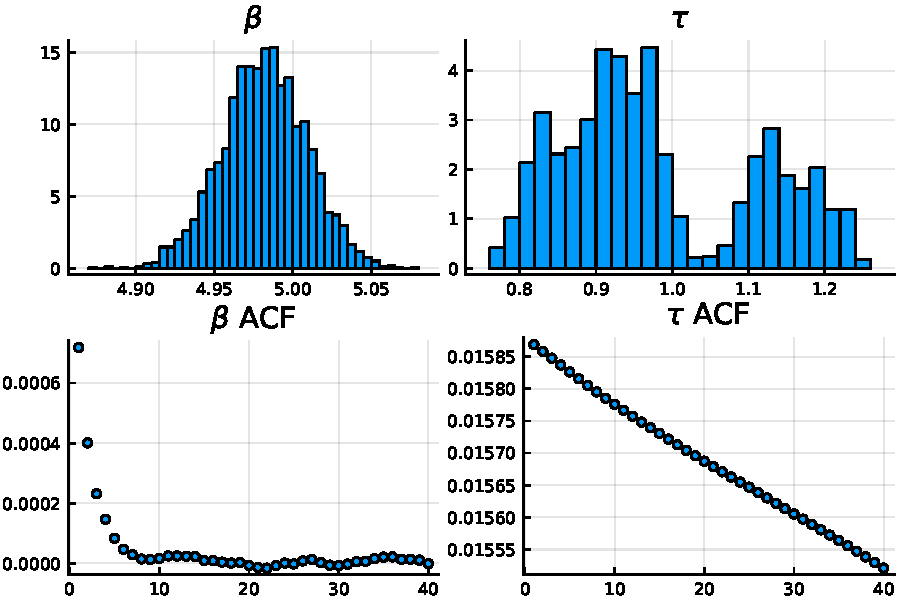
\includegraphics[width=.9\linewidth]{./Linear.pdf}
  \caption{Pseudo-Marginal MCMC Linear Link}
\end{figure}

For the pseudo-marginal MCMC simulation, I found that there was a 35\%
acceptance probability for the distribution, and the auto-correlation
function is shown as well.

\begin{figure}[h!]
  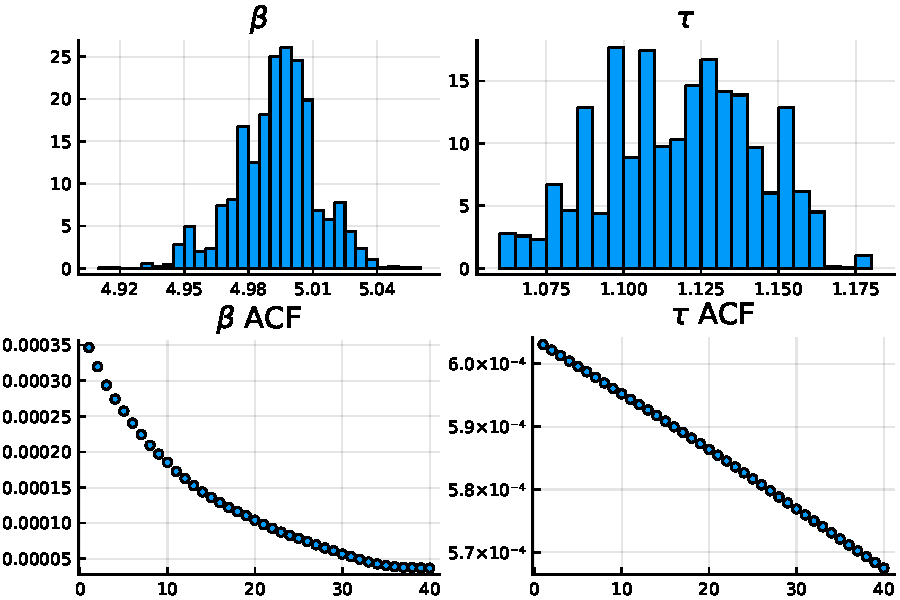
\includegraphics[width=.9\linewidth]{./Linear_A.pdf}
  \caption{Metropolis-Hastings Linear Link}
\end{figure}

For the single $\alpha$ sample (algorithm A), I found that there was a
significantly lower acceptance probability (5\%). This led to a much
poorer mixture. However, the mixture under the pseudo-marginal MCMC is
still not ideal, as there is quite a bit of noise in the distribution
of $\tau$ despite the prior being a normal distribution, and the data
being simulated from a normal distribution.

It is likely that this problem could be resolved by a better choice of
sampling than the plain Monte-Carlo integration employed in the
suggestion. If the points were suggested based on some form of
Gaussian quadrature or importance sampling, there could be a much
better mixture distribution for the taus.

For testing the Logistic link function, I sampled the distribution of
the $Y$ by using $Y_{i,t} \sim bernoulli( g( X_{i,t}\beta + \alpha_i))$ where $g$
is the inverse of the logit function. This is the standard link
function for logistic regression. Conditional on $\beta,\alpha$ the likelihood
function is then given by:
\begin{equation*}
  L = \prod_{i=1}^I \prod_{t=1}^T y_{i,t} log( g( X_{i,t}\beta + \alpha_i)) +
  (1-y_{i,t}) log( 1 - g(X_{i,t}\beta + \alpha_i))
\end{equation*} 

Using Algorithm A, I find a much better mixing probability than the
under the linear model, which is likely because I do not simulate the
model under any noise, and only round up or down based on the
inverse-logit transformation. I find an acceptance probability of
41\%. The distribution for $\tau$ is quite different, with much of its
mass to the left of the mode rather than a symmetric distribution that
was expected. 

\begin{figure}[h!]
  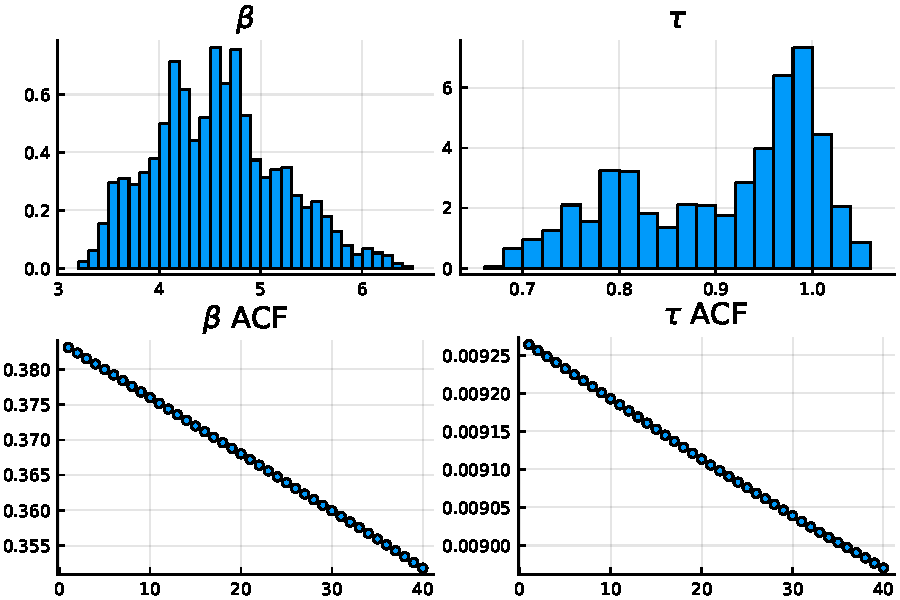
\includegraphics[width=.9\linewidth]{./Logit_A.pdf}
  \caption{Logistic Algorithm A}
\end{figure}

For the pseudo-marginal MCMC sampler of the distribution in the
logistic, the distribution is far less ideal. The estimate for $\beta$ has
most of its mass away from the true value that the simulated data is
based around. While the $\beta$ estimate is underestimated, the $\tau$ is
overestimated to attempt to compensate. I find that there is an
extremely high acceptance rate of $95\%$, which is up quite a lot from
the linear case, though the correlation is much higher as well. This
indicates that there is not as much exploration of the distribution,
and that it is not mixing as well as it should.

\begin{figure}[h!]
  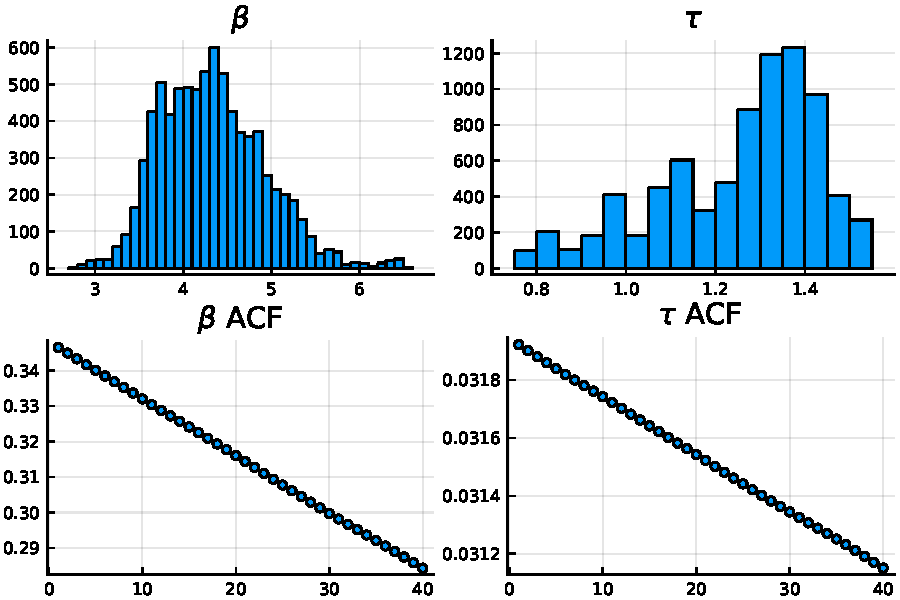
\includegraphics[width=.9\linewidth]{./Logistic.pdf}
  \caption{Logistic Pseudo-Marginal MCMC}
\end{figure}

In this case, we see that the MCMC actually performs better than the
pseudo-marginal MCMC sampler for this distribution. This is for a
relatively large sample, and a large size for the MCMC as well as a
large number of samples for $\alpha$.

If we consider the linear case, and wish to figure out the
distribution of the likelihood function, we may calculate the
likelihood values for the sampled values of $\beta,\tau$.


\end{document}
